\documentclass[12pt]{article}
\usepackage{worksheet-common}

% Test 4 review practice. Modeled on the harder problems from Written HW 7
% & HW 8 (magnetic fields, forces, and particle motion, Part A below) and
% Written HW 9 (flux, Faraday's law, Lenz's law, and induced fields, Part B
% below) -- same problem types, new numbers, so working them actually
% requires redoing the steps. Every formula used here is on the Magnetism
% equation sheet (Knight ch. 29-30); Part A pairs stick to the sheet's
% "derived -- given results, use these directly" formulas (straight wire,
% center-of-loop field, not the general on-axis-at-distance formula, which
% isn't on the algebra-track sheet). Within each pair the SECOND problem
% solves for a different unknown than the first, same as the Test 3 set.
%
% 2026-11-12, at Seth's request ("Part A a little harder ... some dipole
% questions, including torque and PE"): the two single-wire plug-ins became
% two-wire superposition problems (HW 7's 29.13 type), the coil pair gained
% a torque / energy part each, and problems 5-6 are new dipole torque and
% orientation-energy problems (sheet Sec. 4: m = NIA, tau = m B sin(theta),
% U = -m B cos(theta); dipole moment is m, not mu, per Seth 2026-11-12). Problem 5 gives the angle of the coil's PLANE on
% purpose. Part A is now 10 problems; Part B is 11-18.

\begin{document}

\worksheettitle{Test 4 Practice --- Magnetism \& Induction}

\noindent These are modeled on the hardest problems from Written HW 7, HW
8, and HW 9 -- same problem types, new numbers. Every formula you need is
on the Magnetism equation sheet; have it open while you work. Each pair of
problems below tests the same idea but asks for a different unknown, so
skim the whole question before you start plugging in. The answer key is on
the last page.

%============================================================
\partsec{A}{Magnetic Fields, Forces \& Motion}

\prob Two long, straight, parallel wires are 10 cm apart. Wire 1, on the
left, carries 15 A out of the page; wire 2, on the right, carries 25 A
into the page. (a) Find the magnitude and direction of the magnetic field
at point $P$, midway between the wires. (b) At what point on the line
through the two wires is the magnetic field zero?

\begin{center}
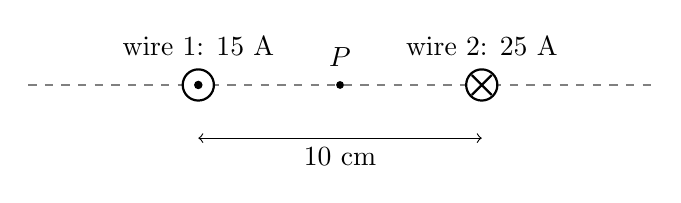
\begin{tikzpicture}[scale=0.9]
  \draw[gray,dashed] (-2.4,0)--(6.4,0);
  \filldraw[thick,fill=white] (0,0) circle (0.22); \fill (0,0) circle (0.06);
  \filldraw[thick,fill=white] (4,0) circle (0.22);
  \draw[thick] (3.86,-0.14)--(4.14,0.14) (3.86,0.14)--(4.14,-0.14);
  \node[above=7pt] at (0,0) {wire 1: 15 A};
  \node[above=7pt] at (4,0) {wire 2: 25 A};
  \fill (2,0) circle (0.055) node[above=3pt]{$P$};
  \draw[<->] (0,-0.75)--(4,-0.75) node[midway,below]{10 cm};
\end{tikzpicture}
\end{center}

\worksp{sm}

\prob Two long, straight, parallel wires are 7.0 cm apart and carry
currents in the \emph{same} direction. Wire 1 carries 8.0 A. The magnetic
field is zero at a point between the wires, 2.0 cm from wire 1. (a) What
current flows in wire 2? (b) What is the magnetic field strength at the
point midway between the wires?

\worksp{7cm}

\prob A 50-turn circular coil of radius 4.0 cm carries a current of 2.0 A.
Find (a) the coil's magnetic dipole moment, (b) the magnetic field
strength at the center of the coil, and (c) the largest torque the coil
can feel when it is placed in a uniform 0.30 T magnetic field.

\worksp{lg}

\prob A single-turn circular loop of radius 3.0 cm carries current $I$.
The magnetic field at the loop's center is measured to be 42 $\mu$T.
(a) What current flows in the loop? (b) What is the loop's magnetic dipole
moment? (c) The loop is now placed in a uniform 0.80 T external field. In
which orientation is its potential energy greatest, and what is the
potential energy in that orientation?

\worksp{lg}

\prob A rectangular 20-turn coil, 5.0 cm $\times$ 8.0 cm, carries a
current of 1.5 A. It sits in a uniform 0.40 T magnetic field, and the
\emph{plane} of the coil makes a $60^\circ$ angle with the field. Find (a)
the magnitude of the torque on the coil, and (b) the coil's potential
energy. (c) The coil is released and turns until its dipole moment lines
up with the field. By how much does its potential energy change?

\worksp{lg}

\prob A small bar magnet feels a torque of 0.036 N$\cdot$m when its axis
is at $35^\circ$ to a uniform 0.15 T magnetic field. (a) What is the
magnitude of the magnet's dipole moment? (b) How much energy does it take
to turn the magnet from pointing along the field to pointing opposite the
field? (c) At what angle from the field is the magnet's potential energy
$+0.025$ J?

\worksp{lg}

\prob An electron travels at $2.0\times10^6$ m/s between two parallel
plates separated by 2.0 cm and charged by a 400 V battery (top plate
positive). What magnetic field strength and direction will let the
electron pass between the plates without being deflected?

\worksp{lg}

\prob An antiproton (same mass as a proton, $q=-e$) moves at 400 m/s to
the left through a region with uniform fields $\vec E=1500$ V/m (pointing
up, in the plane of the page) and $\vec B=3.0$ T (into the page). Find the
magnitude and direction of the antiproton's acceleration at this instant.

\worksp{lg}

\prob A uniform 40 mT magnetic field points in the $+z$ direction. A
proton enters the field moving at $2.0\times10^6$ m/s, at $40^\circ$ above
the $xy$-plane. Find the radius $r$ and the pitch $p$ of the proton's
helical trajectory.

\worksp{lg}

\prob A proton moves through a uniform 25 mT magnetic field on a helical
path with radius 2.0 cm and pitch 8.0 cm. Find the proton's speed $v$ and
the angle above the $xy$-plane at which it entered the field.

\worksp{xl}

\clearpage
%============================================================
\partsec{B}{Electromagnetic Induction}

\prob A 15-cm-long wire is pulled along a U-shaped conducting rail in a
perpendicular magnetic field. The total resistance of the wire and rail is
0.40 $\Omega$. Pulling the wire at a steady speed of 3.0 m/s causes 6.0 W
of power to be dissipated in the circuit. Find (a) the pulling force, and
(b) the magnetic field strength.

\worksp{md}

\prob A 20-cm-long wire slides along a U-shaped conducting rail in a 1.5 T
field perpendicular to the rail's plane, pulled at a constant 5.0 m/s. The
total resistance is 0.60 $\Omega$. Find (a) the induced emf and current,
(b) the power dissipated, and (c) the pulling force required.

\worksp{lg}

\prob A square conducting loop, 15 cm on each side, is positioned so that
exactly 60\% of its area lies within a 0.25 T magnetic field (directed
into the page); the rest of the loop is in a field-free region. (a) What
is the magnitude of the magnetic flux through the loop? (b) If the field
strength \emph{increases}, what is the direction of the induced current in
the loop?

\worksp{lg}

\prob A bar magnet's south pole is pushed toward a stationary conducting
loop, face-on. As the magnet approaches, is a current induced in the
loop? If so, use Lenz's law to determine whether the near face of the
loop becomes a north or south magnetic pole.

\worksp{md}

\prob A 500-turn coil of wire 2.0 cm in diameter sits in a magnetic field
that increases from 0.050 T to 0.200 T in 25 ms. The coil's axis is
parallel to the field. What is the induced emf of the coil?

\worksp{md}

\prob A 50-turn coil, 4.0 cm in diameter, has a resistance of 2.0
$\Omega$. A magnetic field perpendicular to the coil increases at a
steady rate of 0.80 T/s. Find (a) the induced emf, and (b) the induced
current.

\worksp{lg}

\prob The magnetic field inside a circular region of radius 4.0 cm points
into the page and is decreasing at the rate 0.25 T/s. (a) What is the
magnitude of the induced electric field at a point 2.0 cm from the
center? (b) Is the induced electric field clockwise or counterclockwise?
(c) A proton released from rest at that point momentarily feels a force.
What is the magnitude of its initial acceleration?

\worksp{lg}

\prob At a point 5.0 cm from the center of a circular field region, the
induced electric field has magnitude 0.030 V/m. (a) At what rate is the
magnetic field changing? (b) An electron released from rest at a point
2.0 cm from the center (same field region) feels what initial
acceleration?

\worksp{lg}

\begin{answerkey}
\begin{multicols}{2}

\akpart{Part A --- Magnetic Fields, Forces \& Motion}
\akitem{1}{(a) $B=B_1+B_2=60\ \mu\text{T}+100\ \mu\text{T}=160\ \mu$T,
toward the top of the page\quad (b) 15 cm to the left of wire 1 (25 cm
from wire 2)}
\akitem{2}{(a) $I_2=20$ A\quad (b) $B=114\ \mu\text{T}-46\ \mu\text{T}
\approx69\ \mu$T}
\akitem{3}{(a) $m=NIA=0.50\ \text{A}\cdot\text{m}^2$\quad (b) $B=1.6$ mT\quad
(c) $\tau_{\max}=mB=0.15$ N$\cdot$m}
\akitem{4}{(a) $I=2.0$ A\quad (b) $m=5.7\times10^{-3}\
\text{A}\cdot\text{m}^2$\quad (c) $\vec m$ opposite to $\vec B$;
$U=+mB=4.5$ mJ}
\akitem{5}{$m=NIA=0.12\ \text{A}\cdot\text{m}^2$, and $\vec m$ is
$30^\circ$ from $\vec B$ (it is perpendicular to the coil's plane)\quad
(a) $\tau=0.024$ N$\cdot$m\quad (b) $U=-0.042$ J\quad (c) it drops by 6.4
mJ ($\Delta U=-6.4\times10^{-3}$ J)}
\akitem{6}{(a) $m=0.42\ \text{A}\cdot\text{m}^2$\quad (b) $\Delta
U=2mB=0.13$ J\quad (c) $\theta\approx113^\circ$}
\akitem{7}{$B=10.0$ mT, into the page}
\akitem{8}{$F_{\text{net}}=4.8\times10^{-17}$ N, down; $a=2.9\times10^{10}\
\text{m/s}^2$, down}
\akitem{9}{$r=0.40$ m; $p=2.1$ m}
\akitem{10}{$v\approx5.7\times10^4$ m/s; $\theta\approx33^\circ$}

\akpart{Part B --- Electromagnetic Induction}
\akitem{11}{(a) $F_{\text{pull}}=2.0$ N\quad (b) $B\approx3.4$ T}
\akitem{12}{(a) $\mathcal{E}=1.5$ V, $I=2.5$ A\quad (b) $P=3.75$ W\quad (c)
$F_{\text{pull}}=0.75$ N}
\akitem{13}{(a) $\Phi\approx3.4\times10^{-3}$ Wb\quad (b)
counterclockwise}
\akitem{14}{Yes; the near face becomes a south pole (repelling the
approaching magnet)}
\akitem{15}{$\mathcal{E}\approx0.94$ V}
\akitem{16}{(a) $\mathcal{E}\approx50$ mV\quad (b) $I=25$ mA}
\akitem{17}{(a) $E=2.5\times10^{-3}$ V/m\quad (b) clockwise\quad (c)
$a\approx2.4\times10^5\ \text{m/s}^2$}
\akitem{18}{(a) $|dB/dt|=1.2$ T/s\quad (b) $a\approx2.1\times10^9\
\text{m/s}^2$}

\end{multicols}
\end{answerkey}

\end{document}
